\documentclass[sigconf,review=true]{acmart}

%\begin{CCSXML}
%	<ccs2012>
%	   <concept>
%		   <concept_id>10011007.10011006.10011072</concept_id>
%		   <concept_desc>Software and its engineering~Software libraries and repositories</concept_desc>
%		   <concept_significance>500</concept_significance>
%		   </concept>
%	 </ccs2012>
%\end{CCSXML}
%	
%\ccsdesc[500]{Software and its engineering~Software libraries and repositories}
\keywords{data layout, data optimization, loop chains, inter-loop optimization, performance model}
\usepackage{array} 
\usepackage{comment}
\usepackage{graphicx}
\usepackage{csquotes}
\usepackage{balance}
\usepackage{setspace}

\usepackage{listings}
\usepackage{lstautogobble}
\usepackage{subcaption}

\usepackage{standalone}
\usepackage{algorithmicx}

\lstset{ %
language=C++,                % choose the language of the code
basicstyle=\ttfamily\footnotesize,       % the size of the fonts that are used for the code
columns=fullflexible,
numbers=left,                   % where to put the line-numbers
numberstyle=\footnotesize,      % the size of the fonts that are used for the line-numbers
stepnumber=1,                   % the step between two line-numbers. If it is 1 each line will be numbered
numbersep=5pt,                  % how far the line-numbers are from the code
%backgroundcolor=\color{codeBG3},  % choose the background color. You must add \usepackage{color}
showspaces=false,               % show spaces adding particular underscores
showstringspaces=false,         % underline spaces within strings
showtabs=false,                 % show tabs within strings adding particular underscores
frame=single,           % adds a frame around the code
tabsize=2,          % sets default tabsize to 2 spaces
captionpos=b           % sets the caption-position to bottom
breaklines=true,        % sets automatic line breaking
breakatwhitespace=false,    % sets if automatic breaks should only happen at whitespace
keywordstyle=\color{blue},       % keyword style
  %language=Octave,                 % the language of the code
  otherkeywords={SearchVar,MV,TSS,tileExpr,Search,tFunc...},           % if you want to add more keywords to the set
  numberstyle=\tiny\color{black}, % the style that is used for the line-numbers
  rulecolor=\color{black},
escapeinside={<@}{@>}
} 
\definecolor{ForestGreen}{RGB}{34,139,34}
\newcommand{\todo}[1]{{\textcolor{red}{{\tt{TODO:}}\,\,#1 }}}
\newcommand{\nc}[0]{\todo{cite}}
\newcommand{\an}[1]{{\textcolor{blue}{Author's Note: #1}}}
\newcommand{\ttt}[1]{{\texttt{#1}}}

\newcommand{\FormatDecisions}[0]{{\texttt{FormatDecisions}}~}

\graphicspath{{.}{ScoreValidity}{RAJAPerf}}

%\usepackage[subtle]{savetrees}
\vbadness=18000
\vfuzz=2pt
\title{Data Layout Optimization in RAJA}


% \author{Brandon Neth}
% \affiliation{%
% 	\institution{University of Arizona}
% 	\city{Tucson}
% 	\state{AZ}
% 	\country{USA}}
% \email{brandonneth@email.arizona.edu}

% \author{Thomas R.W. Scogland}
% \affiliation{
% 	\institution{Lawrence Livermore National Laboratory}
% 	\city{Livermore}
% 	\state{CA}
% 	\country{USA}}

% \author{Bronis R. de Supinski}
% \affiliation{
% 	\institution{Lawrence Livermore National Laboratory}
% 	\city{Livermore}
% 	\state{CA}
% 	\country{USA}}

% \author{Michelle Mills Strout}
% \affiliation{%
% 	\institution{University of Arizona}
% 	\city{Tucson}
% 	\state{AZ}
% 	\country{USA}}




\begin{document}



\begin{abstract}

The layout of data in memory is a key consideration in high performance computing applications.
From reducing cache and page misses to relieving pressure on memory bandwidth and avoiding inter-process communication, a good data layout improves performance at all levels of an application.
RAJA, a C++ performance portability library, incorporates the layout of an application's data into its interface.
Thus, a developer can try different layouts without major refactoring costs.
However, some applications benefit from changing the data layout mid-computation to facilitate better locality.
Implementing such a mid-computation layout change in RAJA can improve performance, but is laborious to implement and lacks portability.
This work remedies RAJA's shortcoming by introducing a lightweight, declarative API for changing data layouts between computations.
We then extend the library with existing compiler technology to guide the use of layout changes based on our runtime performance model of their cost and benefit.
Thus, the model and runtime combine to \enquote{fill in} layout choices that the user did not specify.
Our approach allows the user to specify as much of the layout information as they please and still obtain the performance benefits of changing data layouts.  
Further, our system is built directly into the RAJA library, meaning that no additional build steps are required.
We evaluate our system on four benchmarks, where it achieves similar performance improvements to hand-implemented optimizations.
\end{abstract}
\maketitle
\def\@textbottom{\vskip \z@ \@plus 1pt}




\section{Introduction}

How data is stored and accessed has always been recognized to have a significant impact on performance. 
For example, on a typical cache-based system, iterating through a two-dimensional array in column-order when data is 
stored in row-order can lead to significant slowdown 
Although mechanisms such as compiler optimizations (loop permutation/interchange) 
and data layout policies like those in Kokkos~\cite{edwards2014kokkos} and RAJA~\cite{hornung2014RAJA} can align data layout with computation schedules, they become difficult to automate and laborious to manage by hand as the number of loops and arrays grow.

In this paper, we present an approach for exposing data layout decisions to the programmer in the C++ portable, parallel library RAJA.
The presented API allows the programmer to specify as many data layout decisions in a sequence of data-sharing loops (otherwise known as a loop chain~\cite{krieger2013loop}) as they choose.
Then, using a portable cost model based on microbenchmarking, our system identifies any remaining layout changes estimated to improve performance.  

Figure~\ref{IntroExample} shows the importance of a good data layout. 
The BadLayout column shows the execution time for a matrix multiplication where the three arrays are laid out opposite of their access order. 
The GoodLayout column shows the execution time for the same matrix multiplication when the arrays are laid out to match their access order.
The LayoutChange column shows the execution time of code that changes the layout from the bad layout to the good one.
Finally, the SwitchAndRun column shows the combined execution time of changing the layout from bad to good and then running.
As the graph shows, performance improves  significantly (72\%) simply by changing the data layout, and the cost of performing the layout change is small (<1\% of execution time). 

\begin{figure}
	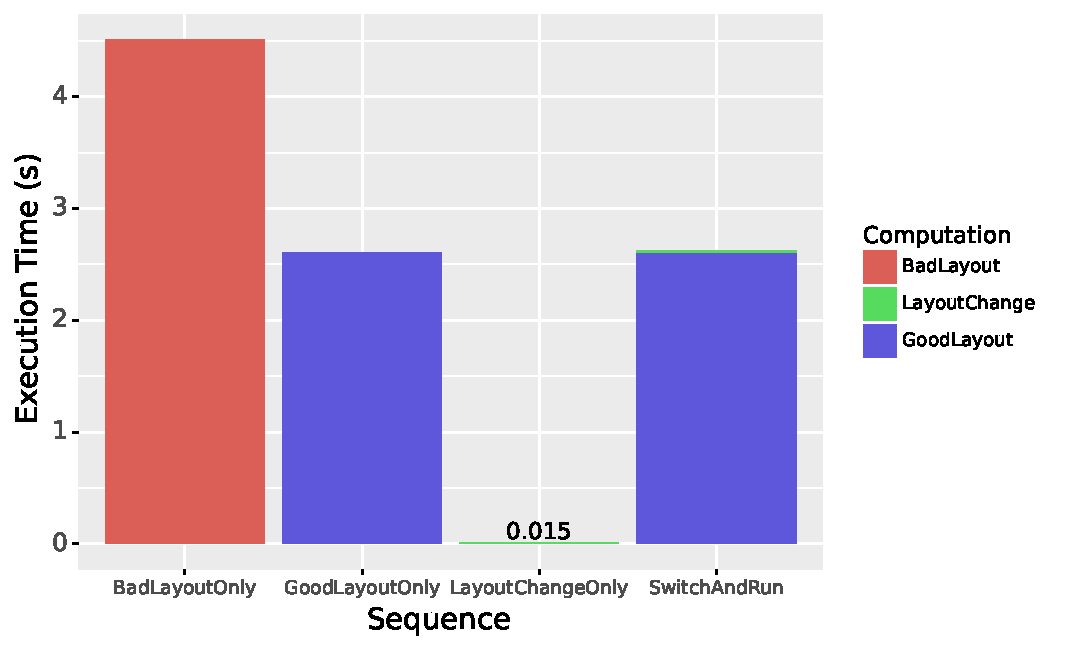
\includegraphics[width=\columnwidth]{IntroExampleGraph.pdf}
	\caption{Execution time for matrix multiplication using optimal and non-optimal data layouts and execution time for converting from non-optimal to optimal.}
	\label{IntroExample}
	\Description[Matrix Multiplication Execution Time for Different Layouts]{A bar plot showing a "Bad Layout" column with execution time greater than the "Good Layout" and "Layout Conversion" columns combined.}
\end{figure}




General purpose libraries like Kokkos and RAJA and programming languages like Chapel~\cite{diaconescu2007approach} give programmers some control over the data layout of multi-dimensional arrays. However, this support is limited to the point of initialization.
Thus, programmers must use that particular data format for the entire computation.
While a developer could change the data layout mid-computation in RAJA, the developer must either modify RAJA library code or use multiple arrays for the same data. 
Both options increase the code complexity and increase its fragility.
Even for the brave developer choosing one of these options, yet another obstacle remains: selecting the right combination of formats for the computation.
Even a modest computation of two loops using four 2D arrays has more than 200 combinations from which to choose, meaning trying out all possible options quickly becomes infeasible. 

There is a significant body of work that developed ILP problems for determining data layouts in distributed memory settings for programming languages like HPF and D~\cite{bixby1994automatic,kennedy1995automatic,kennedy1998automatic}. 
A similar line of work~\cite{chen2004ilp,chen2005constraint,chen2005integrating, ozturk2011data} uses ILP-based constraint networks to combine data layout and schedule optimizations. 
Both of these approaches were developed in the context of a compiler. 
An important idea from this work we build on are automating data layout decisions (partially or fully) through the use of a performance model encoded as the objective function in an ILP problem.
They key difference is that we are providing this data layout compiler technology to the user through a library interface, rather than applying it automatically in a compiler. 
As such, there are advantages to exposing more control to the user. 
There are additional challenges as well: a library needs to do its analysis and decision making at runtime and the interface provided to the user should be high-level while still providing enough control. 
These challenges lead to a number of sub problems such as interface design so that the library implementation can do the analysis needed and quickly enough while maintaining ease of use.
A compiler approach can take longer and has all of the information that the language semantics provide.
Some advantages of a library approach are that it is more accessible to users and the library implementation will have more information available, such as loop bounds, accessible at runtime before a loop executes.
Although useful advantages, these lead to further sub problems about how the library implementation can most leverage the compiler of the language it is embedded in (C++ here) to force as much specialization as possible to achieve the ultimate goal of performance.

We extend the RAJA C++ library to address this gap in support for data layout optimizations.
First, our extension exposes a lightweight API for implementing mid-computation data layout optimizations.
For those with specific format changes in mind, two methods --- \verb.set_format_before. and \verb.set_format_after. --- ensure the appropriate format is used\footnote{Since the control is completely exposed, an autotuner can also try out different options.}.
While the user can specify as many format requirements as they desire, any left unspecified are completed using a performance model.
Guided by run-time microbenchmarking, the model selects format changes based on the solution of an Integer Linear Programming~(ILP) problem that considers the cost of converting formats against the potential improvement with an alternative format.
Our inclusion of a performance model means a developer can obtain performance improvement without having to determine the sequence of format changes themselves or use an autotuner to try every possible option.

This paper includes the following contributions:
\begin{itemize}
\item An API in RAJA for specifying data layouts and data layout transformations;
\item A performance model to select data layouts based on runtime microbenchmarking and a data layout transformation strategy for a loop chain;
\item An optimization that increases the reuse of microbenchmarking information; and
\item Performance results and source lines of code (SLOC) for five variants of four benchmark kernels comparing hand-implemented optimizations to our system.
\end{itemize} 


%%%%%%%%%%%%%%%
\section{RAJA and RAJALC}

\begin{figure}
	\begin{lstlisting}[
		caption={The running example for this paper. 
		We start with an implementation of the 3MM kernel (E = A * B, F = C * D, G = E * F) in RAJA.},
		label={3MMStart}]
	auto layout_01 = make_permuted_layout(sizes, {{0,1}});
	auto layout_10 = make_permuted_layout(sizes, {{1,0}});
	View2D A(A_data, layout_01);
	View2D B(B_data, layout_10);
	... initializations proceed similarly for C-G with layout_01

	auto loop_body1 = [&](auto i0, auto i1, auto i2) {
		E(i0, i1) += A(i0,i2) * B(i2,i1);
	};
	auto loop_body2 = [&](auto i0, auto i1, auto i2) {
		F(i0, i1) += C(i0,i2) * D(i2,i1);
	};
	auto loop_body3 = [&](auto i0, auto i1, auto i2) {
		G(i0, i1) += E(i0,i2) * F(i2,i1);
	};
	
	using POLICY = KernelPolicy<
		statement::For<0,omp_parallel_for_exec,
			statement::For<1,loop_exec,
				statement::For<2,loop_exec,
					statement::Lambda<0>
				>
			>
		>
	>;

	auto one_seg = RangeSegment(0,N);
	auto segs = make_tuple(one_seg, one_seg, one_seg);

	auto knl1 = make_kernel<POLICY>(segs, loop_body1);
	auto knl2 = make_kernel<POLICY>(segs, loop_body2);
	auto knl3 = make_kernel<POLICY>(segs, loop_body3);

	knl1();
	knl2();
	knl3();
	\end{lstlisting}
	\Description[RAJA Implementation of 3MM]{Fully described in the text.}
\end{figure}


We use a variety of components of RAJA to enable automatic data format transformations, as well as features of the loop chain extension RAJALC~\cite{neth2021inter}. 
This section reviews how a computation is described in RAJA, working with the implementation of the 3MM kernel found in Listing~\ref{3MMStart}.

The foundational elements of RAJA are the execution constructs, \verb.forall. and \verb.kernel.. 
These templated functions execute a loop immediately, whereas the RAJALC \verb.make_forall. and \verb.make_kernel. extensions create wrapper objects that are executed through the call operator. 
Calls to \verb.make_kernel. can be seen in lines 30 through 32 in Listing~\ref{3MMStart}. 
While the RAJALC functions create computation objects rather than immediately executing the computation, their interfaces are the same as their base RAJA counterparts.

The execution constructs separate the specification of the computation from the specification of its schedule.
The template parameter describes the schedule of the computation as an execution policy, defined on lines 17 through 25.
Each level of the loop has its own schedule, where \verb.omp_parallel_for_exec. indicates an OpenMP parallel loop and \verb.loop_exec. indicates the compiler should make the decision.
Other policies exist for vectorization and GPU-offloading.
The runtime parameters describe the computation itself. 
The first parameter is the iteration space for the loop, defined on lines 27 and 28. 
The second parameter is the loop body to execute for each iteration, passed as a lambda.
The three loop bodies are defined on lines 7 through 15.
After the computation objects are created on lines 30 through 32, they are executed through the call operator on lines 34 through 36.

RAJA also provides an array wrapper class called a View.
The View object has a number of capabilities that make it a valuable tool within RAJA codes.
First, Views use the call operator to perform memory accesses. 
By overloading this call operator for symbolic iterator types, RAJALC enabled the runtime symbolic evaluation of kernels that use Views.
RAJALC used the access information gathered from symbolic evaluation to ensure the correctness of its scheduling optimizations.
This work uses RAJALC's runtime symbolic evaluation to inform our performance model.

Second, Views fully parameterize their underlying data formats with the Layout object.
Consider a programmer who wants to switch their data from row-major to column-major. 
Without Views, every access to their data \verb.A[i][j]. has to be changed to \verb.A[j][i]. \textit{and} the definition of the array needs to be changed. 
This is prohibitively expensive, especially when the programmer does not yet know the performance impact of such a decision.
With Views however, the only change the programmer needs to make is to the View's definition: the layout permutation changes from $(0,1)$ to $(1,0)$. 
In Listing~\ref{3MMStart}, \verb.A. is defined with the normal $(0,1)$ layout, but \verb.B. is defined with the $(1,0)$ layout. 
Note that the change in \verb.B.'s layout does not change how it is used in the computation. 




\section{User Specification of Data Format}

Throughout a computation, different parts of the computation access data in different orders.
For example, consider the Views \verb.A., \verb.B., and \verb.D. in Listing~\ref{3MMStart}. 
The order in which \verb.A. is accessed is different from \verb.D. because the argument order in their accesses are different.
In contrast, while \verb.B. and \verb.D. have the same argument order, their access order is still different because they have different layouts.
Looking at the two references to \verb.F. in kernels two and three, we can see that even access order to the same data can change through a computation.
Because different formats are optimal for different kernels, this creates an opportunity for optimization. 

However, RAJA's built-in support for changing data layouts is minimal. 
While Views can be instantiated with different layouts, changing the layout of an existing View is not as simple.
This is because changing layouts also requires reordering the underlying data to match the new layout. 
To implement such a layout change by hand requires the programmer to allocate a new temporary array, 
copy the data from the View to the temporary array in the right order, 
copy the data \textit{back} to the memory in the View, 
and then finally update the View's layout object.

This work removes that barrier by expanding the declarative data optimization system begun by RAJALC.
While RAJALC tackled the problem of scheduling optimizations, we target making data format changes between computations. 
The new \verb.FormatDecisions. object is the central component of our system. 
Its instantiation takes a tuple of references to Views that are possible targets of format changes and the kernel objects that constitute the whole computation.
Two methods are used to register desired formats: \verb.set_format_before. and \verb.set_format_after..
Both take the View to be reformatted, the desired format, and the computation before or after which the desired format should be used.
Once all format choices are registered, the complete computation with the desired format conversions is generated using the \verb.finalize. method.


\begin{figure}
\begin{lstlisting}[caption={The 3MM benchmark implemented using FormatDecisions.},
	label={FormatDecisions3MM}]
auto knl1 = make_kernel<KPOL>(segs1, [=](auto i0, auto i1, auto i2) {
	E(i0, i1) += A(i0, i2) * B(i2, i1);
});
auto knl2 = make_kernel<KPOL>(segs2, [=](auto i0, auto i1, auto i2) {
	F(i0, i1) += C(i0, i2) * D(i2, i1);
});
auto knl3 = make_kernel<KPOL>(segs3, [=](auto i0, auto i1, auto i2) {
	G(i0, i1) += E(i0, i2) * F(i2, i1);
});

auto decisions = format_decisions(tie(B,D,F), knl1, knl2, knl3);

decisions.set_format_before(B, {{1,0}}, knl1);
decisions.set_format_before(D, {{1,0}}, knl2);

decisions.set_format_before(F, {{0,1}}, knl1);
decisions.set_format_after(F, {{1,0}}, knl2);

auto computation = decisions.finalize();
computation();
\end{lstlisting}
\Description{Fully described in the text.}
\end{figure}


\section{Performance Modeling}

In addition to the format changes registered by the user, the new \verb.FormatDecisions. also uses a performance model to determine if additional format changes will improve performance. 
This capability means that even without any registered format choices, \verb.FormatDecisions. often selects the same changes the user would themselves choose. 
We encode the problem as an integer linear program where the solution represents our model's pick for the optimal layouts.


We use binary decision variables representing whether or not a particular format is used at different points in the chain. 
For example, there are eight decision variables for the \verb.B. View in Listing~\ref{FormatDecisions3MM}, one for each of the two possible formats at each of the four points in the chain. 
While there are only three kernels in the chain, there is an additional point added for the \enquote{output} format that the View has after the computation is done.
We also add constant variables for the format when the computation begins. 
We also use decision variables to represent the required format conversions.
We construct separate models for each View in the computation. 

Symbolically, we represent the variables as follows.
To start, let $F$, $K$, and $T$ represent the set of all formats, kernels, and conversion times.
Because we add additional elements to $K$ for the input and output formats, we know that $|K|$ is the number of user kernels plus 2.
Furthermore, because there is one more conversion than kernel, we know that $|T| = |K| + 1$.
For each kernel, we have one variable for each format. 
Thus, let $fmt_{f,k}$ denote the variable for using the format $f$ during kernel $k$, where $f \in F$ and $k \in K$.
For conversion variables, we have one variable for each possible conversion at each time point. 
Thus, let $conv_{i,o,t}$ denote the decision variable for converting from format $i$ to to format $o$ at conversion time $t$, where $i,o \in F$ and $t \in T$.

Four types of constraints are imposed on the decision variables.
\begin{itemize}
\item Format Uniqueness: At each time point, the View has exactly one selected format. Given by: 
\begin{align*}
	\bigwedge\limits_{k \in K} (1 = \sum\limits_{f \in F} fmt_{f,k})
\end{align*}
\item Conversion Uniqueness: At each conversion point, the View goes through exactly one conversion. Given by:
\begin{align*}
	\bigwedge\limits_{t \in T} (1 = \sum\limits_{i \in F}\sum\limits_{o \in F} conv_{i,o,t})
\end{align*}
\item Format-Conversion Matching, Input: At each conversion point, the input format for the conversion matches the format of the preceding kernel. Given by:
\begin{align*}
	\bigwedge\limits_{t \in T} \bigwedge\limits_{i \in F} fmt_{i,t.prev} = \sum\limits_{o \in F} conv_{i,o,t}
\end{align*}
\item Format-Conversion Matching, Output: At each conversion point, the output format for the conversion matches the format of the following kernel. Given by:
\begin{align*}
	\bigwedge\limits_{t \in T} \bigwedge\limits_{o \in F} fmt_{o,t.next} = \sum\limits_{i \in F} conv_{i,o,t}
\end{align*}
\item User Prescription: All user-provided format choices are met. With all user choices $U$ represented as pairs of kernels and the format the user wants for that kernel, given by:
\begin{align*}
	\bigwedge\limits_{(k,f) \in U}  fmt_{f,k} = 1
\end{align*}
\end{itemize}
Figure~\ref{ConstraintExample} shows the variables in a model for a 2D View for a computation with three kernels. 
For each kernel, we see two decision variables, one for using column-major and one for using row-major. 
Similarly, for each conversion point, we see four decision variables, one for each combination of input and output format. 
The green boxes indicate the terms that are part of a Format Uniqueness constraint and a Conversion Uniqueness constraint.
The red and blue underline shows the part of the format and conversion decision variables that group them in the Conversion-Format Matching constraints. 

The objective function is constructed using the estimated cost of the format choices and conversions. 
Each decision variable is assigned a cost coefficient in the following manner.
First, we execute and time a small loop with similar access patterns to the choice, then cache the result for later decision variables.
Second, we multiply the result by the number of iterations the choice affects.
For example, a conversion decision for \verb.B. in Listing~\ref{FormatDecisions3MM} would be multiplied by the dimensions of \verb.B..
In contrast, a format decision for \verb.B. for \verb.knl1. would be multiplied by all three loop dimensions. 

While we can estimate the cost of format conversions without information about the kernels themselves, the cost of using a format for a kernel depends on how that kernel accesses the data.
Thus, we need to gather information about how each kernel accesses the data that may be transformed. 
To do so, we use RAJALC's symbolic evaluation capabilities. 
By defining an overloaded call operator in the View class, we can gather access information for each kernel at runtime. 
Then, this access information is used to estimate the cost of using different formats. 
Once all cost estimates are added to the objective function, we use the Integer Set Library~\cite{verdoolaege2010isl} to find the points in the space with the lowest overall cost estimates. 
Listing~\ref{AlgObjFunc} shows a pseudocode algorithm for generating the objective function.
Note that the costs associated with format variables are based on the uses of the Views within the computation. 
Thus, if one kernel makes multiple accesses to the same View, it will have one cost term for each access.


\begin{figure}
\begin{lstlisting}[caption={Algorithm for constructing objective function.}, label={AlgObjFunc}]
add_objective_function(view):
	obj_func = new ObjectiveFunction()
	
	# cost estimates for conversions
	for conversion_variable in conversion_variables:
		coefficient = conversion_variable.estimate_cost() * view.size()
		obj_func += (coefficient * conversion_variable)
	
	# cost estimates for accesses using different formats
	for kernel in kernels:
		view_accesses = kernel.evaluate_symbolically()
		for access to view in accesses:
			for fmt in formats:
				format_variable = get_format_variable(view, fmt, kernel)
				estimated_cost = format_variable.estimate_cost(access)
				coefficient = estimated_cost * kernel.size()
				obj_func += (coefficient * format_variable)
	set_objective_function(obj_func)
\end{lstlisting}
\Description{Algorithm for the function to create the model's objective function. First it adds cost estimates for conversions, then adds cost estimates for the accesses in the computation.}
\end{figure}

\begin{figure*}
	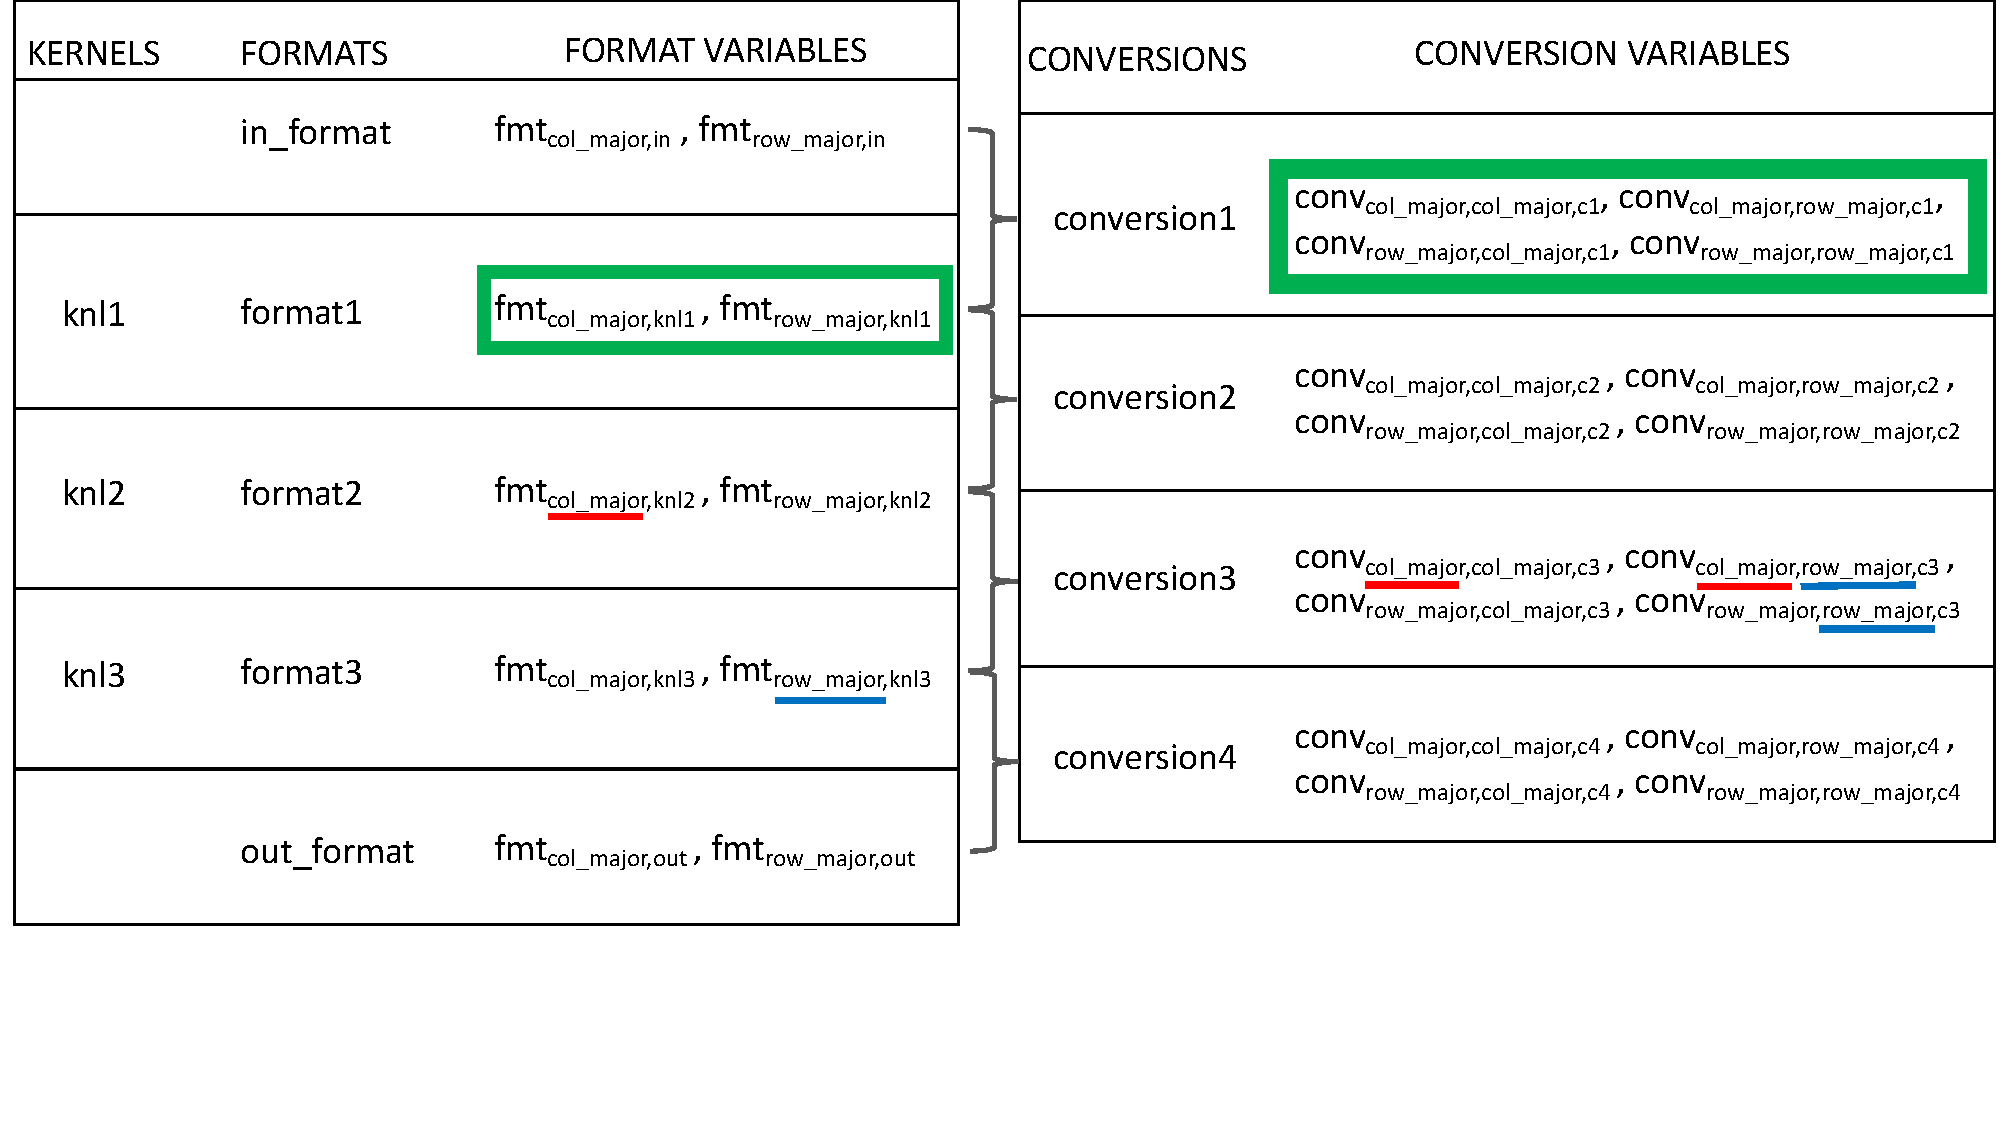
\includegraphics[width=2\columnwidth]{FormatConversionFigure.pdf}
	\caption{Formats, conversions, and decision variables for a 3 kernel computation. The green frames show example groups of variables that must sum to 1 due to the Format and Conversion Uniqueness Constraints. The red and blue underlines show examples of the Conversion-Format Matching constraints for input and output constraints respectively. }
	\label{ConstraintExample}
	\Description{5 columns titled kernels, formats, format variables, conversions, and conversion variables. The conversion columns are offset so that the conversions fall between the formats. A Green box surround the pair of variables fmt col major knl1 and fmt row major knl1. Another green box surrounds the conversion variables for conversion 1.} 
\end{figure*}
\section{Cost Estimation}

Because our system uses microbenchmarking to estimate the cost of different layouts, the overhead can meaningfully impact overall performance. 
To mitigate this effect, we reuse the microbenchmarking results as much as possible.
To maximize reuse, we model choices based on their access order, which describes the order in which iterations access data in memory.

By using the access order instead of the full description of the access, references to different Views can be modeled with the same estimates, even if they have different argument or policy orders.
We argue that the access order is an accurate predictive metric for the relative performance of a layout choice. 

\subsection{Identifying an Access}
\begin{figure}[tbp]
	\begin{lstlisting}[caption={Two implementations of matrix multiplication using different kernel policies.}, autogobble, label={MatMulTraversalOrder}]
		auto a_layout = make_permuted_layout(a_sizes, {{0,1}});
		auto b_layout = make_permuted_layout(b_sizes, {{1,0}});
		auto c_layout = make_permuted_layout(c_sizes, {{0,1}});

		View2D A(a_data, a_layout);
		View2D B(b_data, b_layout);
		View2D C(c_data, c_layout);

		auto matmul_lambda = [&](auto i0, auto i1, auto i2) {
			C(i0,i1) += A(i0,i2) * B(i2,i1);
		}
		auto segs = make_tuple(RangeSegment(0,iN), 
			RangeSegment(0,jN), 
			RangeSegment(0,kN));
		using Policy_012 = KernelPolicy<
			statement::For<0,loop_exec,
				statement::For<1,loop_exec,
					statement::For<2,loop_exec,
						statement::Lambda<0>
					>
				>
			>
		>;

		using Policy_201 = KernelPolicy<
			statement::For<2,loop_exec,
				statement::For<0,loop_exec,
					statement::For<1,loop_exec,
						statement::Lambda<0>
					>
				>
			>
		>;

		auto knl1 = make_kernel<Policy_012>(segs, matmul_lambda);
		auto knl2 = make_kernel<Policy_201>(segs, matmul_lambda);

		knl1();
		knl2();
	\end{lstlisting}
	\Description{Fully described in the text.}
\end{figure}

The access pattern of any View reference is identified by its access order, which is in turn defined by its argument order, the kernel policy order, and the layout order. 
The argument order describes the order of the loop iterators in the reference with respect to the parameters of the lambda. 
In Listing~\ref{MatMulTraversalOrder}, the references to \verb.A., \verb.B., and \verb.C. have argument orders $(0,2)$, $(2,1)$, and $(0,1)$, respectively. 
The kernel policy order describes the order in which the iterators are increased. 
This is equivalent to the nesting order of a loop.
In Listing~\ref{MatMulTraversalOrder}, references made by \verb.knl1. have policy order $(0,1,2)$, while those may by \verb.knl2. have policy order $(2,0,1)$.
The indices of the \verb.For. statements within the policy determine this order.
The layout order describes the layout of data in memory. 
In Listing~\ref{MatMulTraversalOrder}, \verb.A. has layout order $(0,1)$, \verb.B. has $(1,0)$, and \verb.C. has $(0,1)$.
While each access has a layout order defined by the original layout of the data, during our modeling phase, different layout orders are estimated to see which is most effective for the particular kernel. 

The access order describes the order in which the iterations of a kernel access the data in memory.
For example, an access order of $(0,2)$ indicates that the stride-one dimension of the data is traversed by the innermost (depth 2) loop and the larger stride dimension is traversed by the outermost (depth 0) loop. 
Similarly, an order of $(2,1)$ indicates the stride-one dimension is traversed by the middle (depth 1) loop while the larger stride dimension is traversed by the innermost (depth 2) loop.

Calculating the access order of a View reference starts with the argument order.
Then, we permute the argument order based on the layout order. 
Finally, we reorder the result based on the policy order.
Using the reference to \verb.B. in \verb.knl2. as an example, we start with the argument order $(2,1)$.
The layout order of \verb.B. is $(1,0)$, so our intermediate result is $(1,2)$. 
The policy order of \verb.knl2. is $(2,0,1)$, so our final result is $(2,0)$. 
This indicates that in \verb.knl2., the outermost loop is indexing the stride-one dimension while the innermost loop is indexing the larger stride dimension.

Using the access order rather than the full description of the reference, we see that the reference to \verb.B. in \verb.knl1. will have similar performance impact to the reference to \verb.C. in \verb.knl2.
For \verb.B., $(2,1)$ becomes $(1,2)$ becomes $(1,2)$. 
For \verb.C., $(0,1)$ becomes $(0,1)$, becomes $(1,2)$.
This equivalence demonstrates how the monotonically increasing policy and layout orders are identity transformations.

\subsection{Access Order as a Performance Metric}
\label{sec:AccessMetric}
Our claim is that the access order of an access is an accurate predictive metric for the relative performance of a layout choice. 
We support this claim empirically using performance data from three microbenchmarks.
For each microbenchmark, we record the 5-run average execution time of all combinations of policy, layout, and argument order. 
These execution times are then grouped by access order.
If our claim is valid, then the execution times for each access order will cluster and the groups of execution times will not overlap.
Microbenchmark 1 is an access to a 3-dimensional View in a 3-dimensional loop. 
Microbenchmark 2 is an access to a 2-dimensional View in a 3-dimensional loop, as in a matrix multiplication.
Microbenchmark 3 is an access to a 3-dimensional View in a 4-dimensional loop for a set argument order.
Table~\ref{MicrobenchmarkDetails} summarizes them in more detail, including data sizes.
The outermost loop is parallelized using OpenMP.
All evaluation in this paper is performed on the same system. 
We used a single node with two 22-core IBM Power9 CPUs and 256GB of CPU memory.

\begin{table}
	\centering
	\begin{tabular}{p{2.2cm}|p{1.6cm}|p{1.6cm}|p{1.5cm}}

		\raggedright Microbenchmark \linebreak Number & \raggedright \# View \linebreak Dimensions & \raggedright \# Loop \linebreak Dimensions & \raggedright Size per \linebreak Dimension \tabularnewline
		\hline
		1 & 3 & 3 & 128 \\
		2 & 2 & 3 & 512 \\
		3 & 3 & 4 & 64 
	\end{tabular}
	\caption{Microbenchmark details.}
	\label{MicrobenchmarkDetails}
\end{table}

\begin{figure*}
  \centering
  \begin{subfigure}{.48\textwidth}
	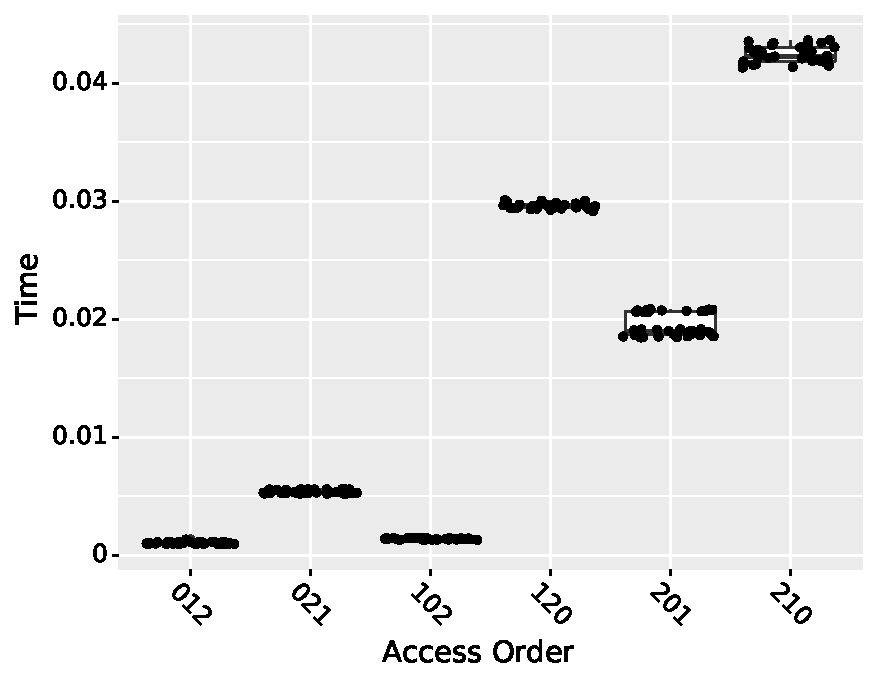
\includegraphics[width=\textwidth]{benchmark1_boxplot.pdf}
	\caption{Box plots showing execution times for 3-dimensional loop accessing 3-dimensional view, grouped by access order. Each point represents a different combination of policy, layout, and argument orders. Each access order group is jittered.}
	\label{AccessBenchmark1}
	\Description[Access Order Execution Times Boxplot for Microbenchmark 1]{Fully described in the text.}
  \end{subfigure}
\begin{subfigure}{.48\textwidth}
	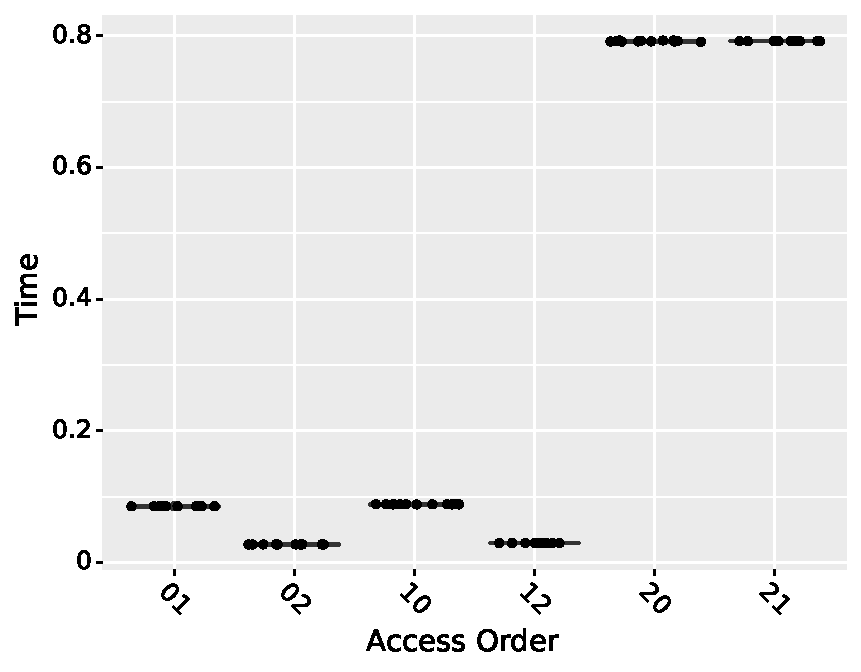
\includegraphics[width=\textwidth]{benchmark2_boxplot.pdf}
	\caption{Box plots showing execution times for 3-dimensional loop accessing 2-dimensional view, grouped by access order. Each point represents a different combination of policy, layout, and argument orders. Each access order group is jittered.}
	\label{AccessBenchmark2}
	\Description[Access Order Execution Time Boxplot for Microbenchmark 2]{Fully described in the text}
\end{subfigure}

\bigskip
\begin{subfigure}{.48\textwidth}
	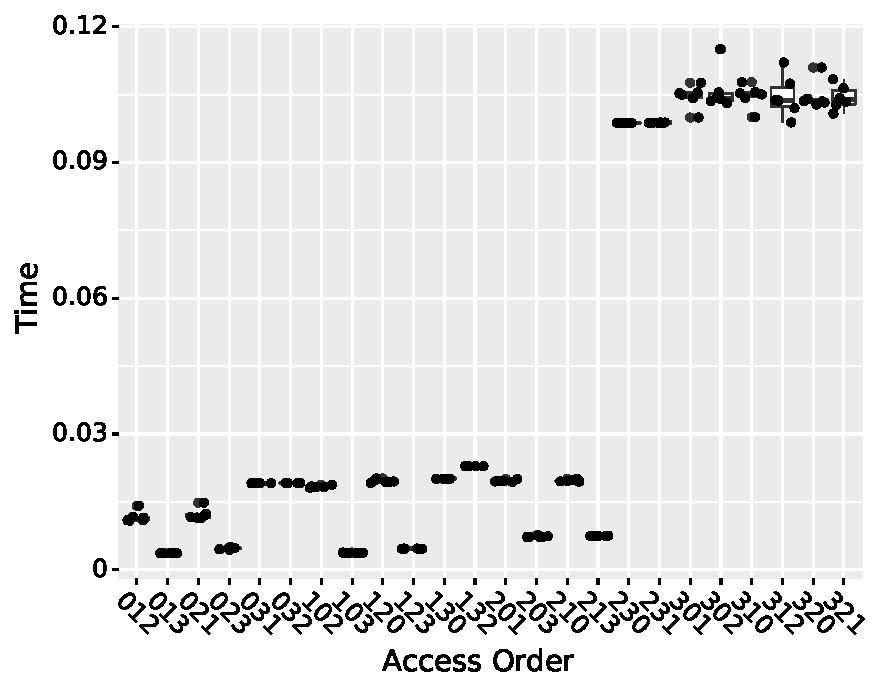
\includegraphics[width=\textwidth]{benchmark3_boxplot.pdf}
	\caption{Box plots showing execution times for 4-dimensional loop accessing 3-dimensional view, grouped by access order. Each point represents a different combination of policy, and layout for a fixed argument order. Each access order group is jittered.}
	\label{AccessBenchmark3}
	\Description[Access Order Execution Time Boxplot for Microbenchmark 3]{Fully described in the text}
\end{subfigure}
\end{figure*}

Figure~\ref{AccessBenchmark1} shows the execution times for the different access orders for microbenchmark 1.
Overall, the six possible access orders show good differentiation and clustering.
The access order $(2,0,1)$ does show two subclusters, but remain highly distinct from the other access order groupings. 
Additionally, access orders $(0,1,2)$ and $(1,0,2)$ show some overlap, likely because the bulk of the performance improvement comes from the innermost loop in a nest traversing the stride-one dimension of the data.
We also hypothesize that the different between orders $(0,2,1)$ and $(2,0,1)$ is due to better data partitioning for the threads in the $(0,2,1)$ order. 
Figure~\ref{AccessBenchmark2} shows the execution times for the different access orders for microbenchmark 2. 
This microbenchmark also shows good cluster and differentiation.
Like microbenchmark 1, the access orders $(0,2)$ and $(1,2)$ have similar performance, likely for the same reason. 
Figure~\ref{AccessBenchmark3} shows the execution times for the different access orders for microbenchmark 3.
A similar pattern as the previous microbenchmarks emerges here: grouping based on the position of the innermost iterator. 


%%%%%%%%%%%%%%%%%%%%%%
\section{Evaluation}

We present a number of experiments to evaluate our system. 
First, we examine performance and productivity using four benchmarks from the polybench suite~\cite{pouchet2012polybench}.
Then, for one of the benchmarks, we perform an exhaustive evaluation of all layout choices to further explore the accuracy of our performance model.
All performance results in this paper were collected on a single node with a 44-core IBM Power9 CPU and 256GB of CPU memory.
All compilation used Clang version 13.0.0.

\subsection{Experiment 1: Polybench}

Our first experiment examined the performance and programmer productivity impacts of our contribution.
We targeted four benchmarks from the Polybench suite: \textsc{2mm}, \textsc{3mm}, \textsc{gemver}, and \textsc{mvt}.
While other benchmarks in the suite have the potential for data layout optimization, they present imperfect nesting and non-constant loop bounds, which are not currently supported by our implementation. 
For each benchmark, we implemented different variants and compared their relative speedup and the number of code changes necessary to go from the original implementation to the variant implementation.
We used RAJAPerf~\cite{hornung2017raja} to run our experiments with default data sizes.

\textsc{2mm} solves the matrix expression $A*B*C$ using two matrix multiplications. 
First, it computes $A*B$ and stores the results in a temporary array.
Then this temporary result is multiplied by $C$.
\textsc{3mm} solves a similar matrix expression $A*B*C*D$ using three matrix multiplications.
It computes $A*B$, then $C*D$, then multiplies the results.
\textsc{gemver} computes a vector multiplication and adds the result to a matrix. 
Finally, \textsc{mvt} computes a \textbf{m}atrix \textbf{v}ector product and \textbf{t}ranspose.

Two of the four benchmarks, \textsc{2mm} and \textsc{3mm}, have higher loop dimensionality than data dimensionality. 
The remaining two, \textsc{gemver} and \textsc{mvt}, have the same loop and data dimensionality. 
This indicates that for \textsc{gemver} and \textsc{mvt}, the most profitable data transformation should be no transformation, as the traversal through the data for the conversion is the same traversal as that of the computation.
For computations such as these, loop schedule transformations may be able to improve locality without the prohibitive cost of format conversions~\cite{kandemir1998improving}.
However, because of their higher loop dimensionality, \textsc{2mm} and \textsc{3mm} should benefit from format conversions.

We implemented five variants of each benchmark.
The first variant, \verb.RAJA_OpenMP., is the original RAJA implementation.
\verb.RAJALC. modifies \verb.RAJA_OpenMP. to use RAJALC kernel objects.
\verb.Hand_Layout., \verb.Format_Decision., and \verb.Model_Choice. all augment the \verb.RAJALC. variant to include format changes.
Table~\ref{VariantDescription} describes the variants in more detail.

\begin{table}
	\centering
	\begin{tabular}{ p{2.4cm} | p{1.1cm} | p{1.1cm} | p{1cm} | p{1cm}}
		 \raggedright Variant \linebreak Name & \raggedright Kernel Objects & \raggedright Layout Changes & \raggedright Chosen By &  Written Using \tabularnewline
		\hline
		\verb.RAJA_OpenMP. & No & No & - & - \\
		\verb.RAJALC. & Yes & No & - & - \\
		\verb.Hand_Layout. & Yes & Yes & User & No API \\
		\verb.Format_Decision. & Yes & Yes & User & API \\
		\verb.Model_Choice. & Yes & Yes & Model & API
	\end{tabular}
	\caption{Polybench variant descriptions.}
	\label{VariantDescription}
\end{table}

\begin{figure}
	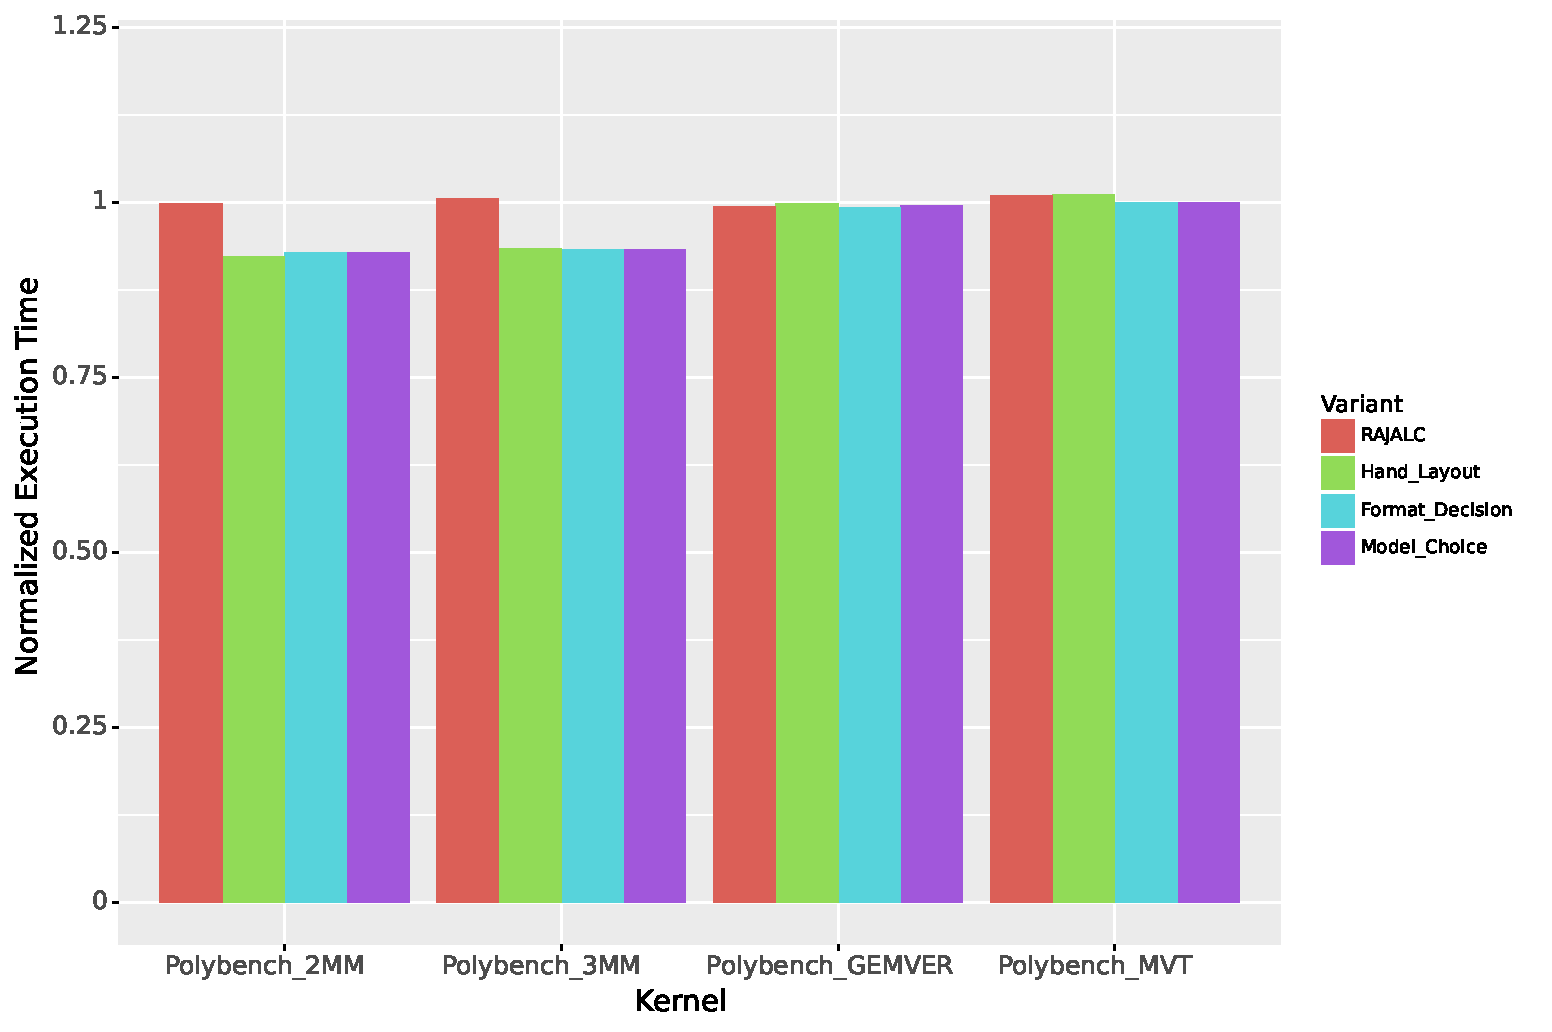
\includegraphics[width=\columnwidth]{PolybenchPerfPlot.pdf}
	\caption{Normalized execution time of the Polybench variants relative to the RAJA\_OpenMP variant (Lower is better). Referent execution times are 3.2,4.7,0.039, and 0.12 seconds.}
	\label{PolybenchPerformance}
	\Description[Polybench Speedups]{Bar chart for the speedup of the different Polybench kernels. Each kernel has a cluster of five bars, one for each variant. }
\end{figure}

Figure~\ref{PolybenchPerformance} reports the average speedup of the variants relative to the \verb.RAJA_OpenMP. variant. 
The average is over 100 runs. 
For the \textsc{2mm} and \textsc{3mm} benchmarks, the results show a meaningful speedup for the three variants that make layout changes (7.7\% to 8.3\% for \textsc{2mm} and 7.0\% to 7.2\% for \textsc{3mm}).
For \textsc{mvt} and \textsc{gemver}, because no layout changes are made, we do not see meaningful performance improvement (<1\% change).
Across all benchmarks, there is little difference performance difference among the variants that make layout changes.
This indicates that the overhead of our system is minimal and that our model makes comparable layout choices to hand-tuning.

To evaluate the productivity of our contribution, we report the source lines of code added or changed for each of the variants.
This value is calculated by counting the number of line differences using python's \verb.Differ.. 
We preprocess to remove all whitespace-only lines.
Figure~\ref{PolybenchSLOC} shows the results.
For the variants that make layout changes, we see a large reduction in the amount of changes required using \verb.FormatDecisions. compared to the by-hand implementation. 
While our tool reduces the code required by more than half, it is important to note that this is with respect to an in-line format conversion.
It is possible for a user to themselves write a function that performs the layout change.
For the variants without layout changes, we see that using \verb.FormatDecisions. can require more code changes than a by-hand implementation. 
This is because the \verb.Hand_Layout. variant is identical to the \verb.RAJALC. implementation, while the \verb.Format_Decision. and \verb.Model_Choice. variants instantiate the \verb.FormatDecisions. object.

\begin{figure}
	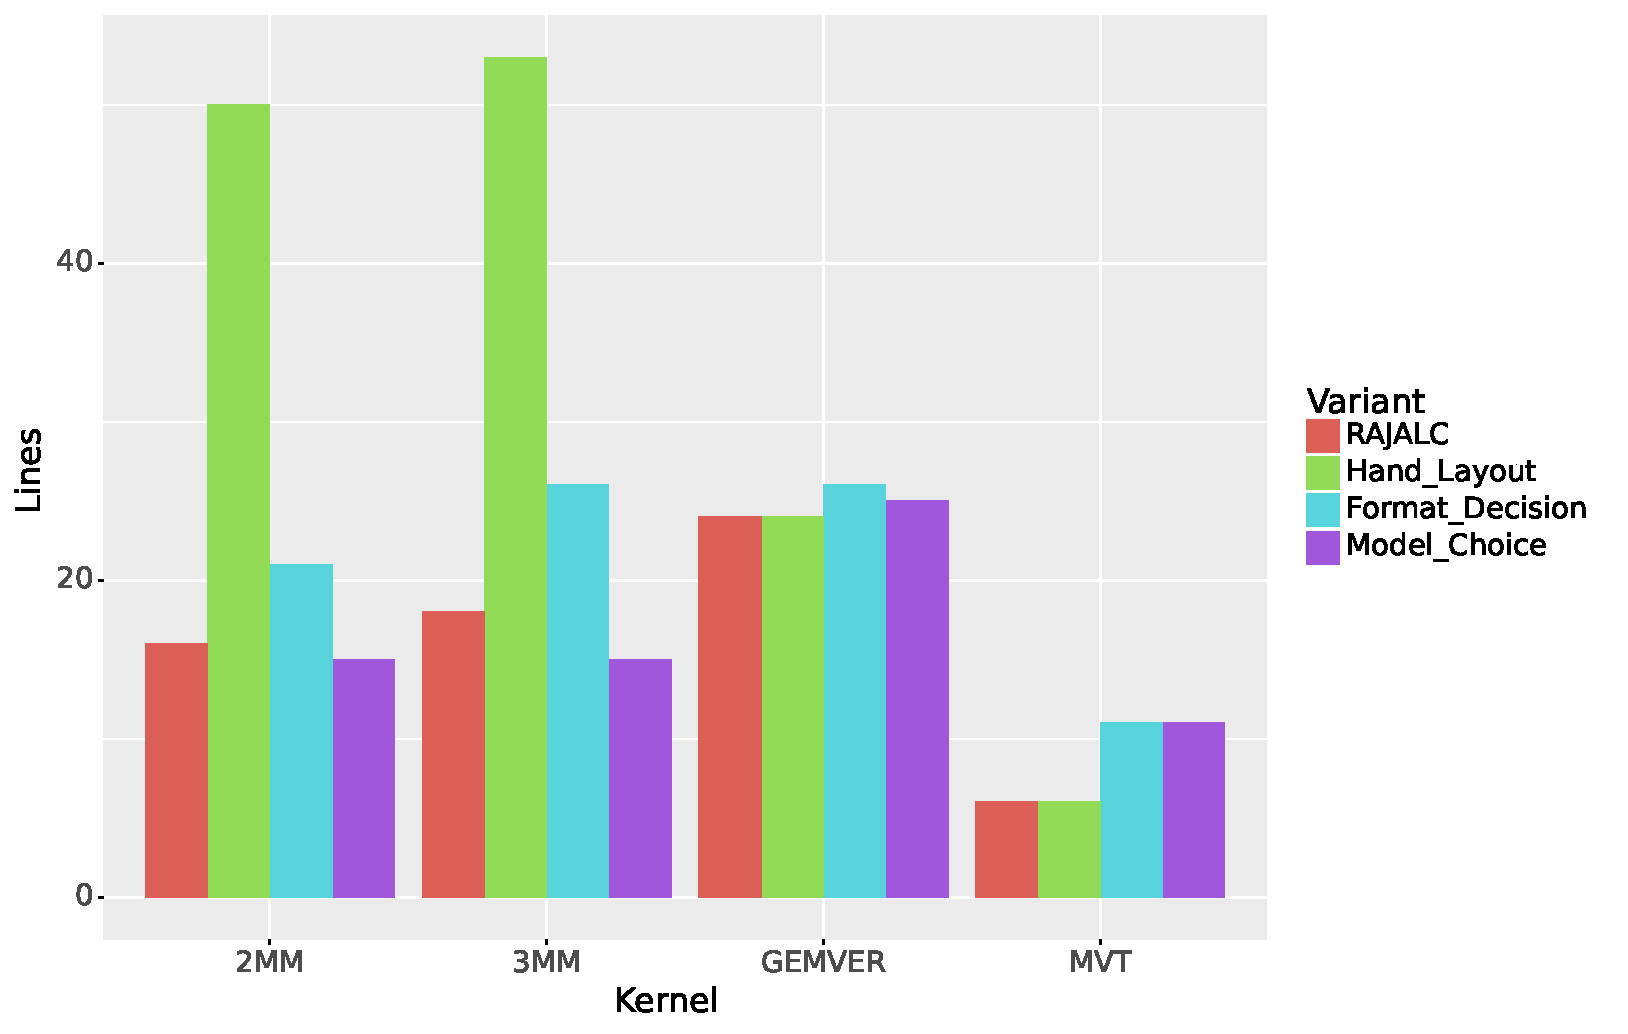
\includegraphics[width=\columnwidth]{PolybenchSLOC.pdf}
	\caption{Source lines of code modified (added, changed, or removed) relative to the RAJA\_OpenMP variant. (Lower is better)}
	\label{PolybenchSLOC}  
	\Description[Polybench SLOC]{Bar chart for the source lines of code changed for the different Polybench kernels. Each kernel has a cluster of four bars, one for each variant that is not the baseline.}
\end{figure}


\subsection{Experiment 2: Exhaustive Search for \textsc{2mm}}

Our second experiment further examines the efficacy of our model. 
Whereas the experiments of in Section~\ref{sec:AccessMetric} examined the efficacy of access order representing individual accesses, this experiment considers the model as a whole.
For the \textsc{2mm} benchmark, we evaluated the performance of all possible format choices and compare their execution times against their model scores (the value of the objective function for that choice).
We average execution times over five runs.
The absolute accuracy of our model is measured by the correlation between the execution time and the model score.
However, we are most interested in the \textit{relative} accuracy of our model.
A model is more relatively accurate when choices with better model scores have lower execution times, regardless of the specific values of the score or execution time.

\begin{figure}
	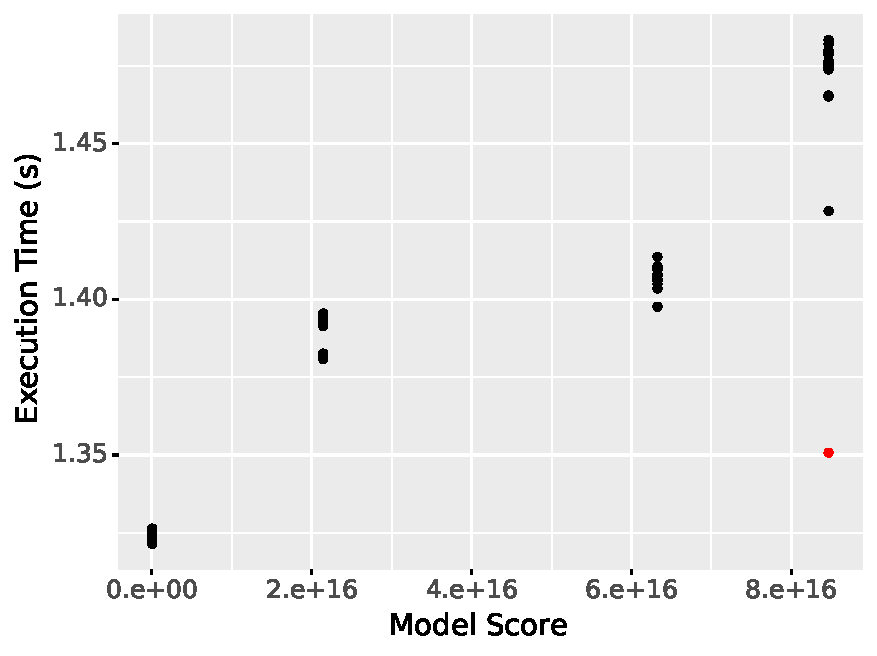
\includegraphics[width=\columnwidth]{2mm-all.pdf}
	\caption{Execution time and model score of all possible format choices for the 2MM kernel. The model selects the choice with the lowest score. Outlier shown in red. All dimension sizes are 1024.}
	\label{2MMAllChoices}
	\Description[Model Score and Execution Time]{Fully described in the text.}
\end{figure}


Figure~\ref{2MMAllChoices} plots the model scores and execution times for the different choices. 
While the overall relationship between model score and execution is as expected, there is one notable outlier, colored in red.
This point, which represents the choice that makes no changes to the data's format, has an unusually high model score for its relatively low execution time. 
This is potentially attributable to our model overestimating the cost of a non-ideal data layout and underestimating the cost of changing formats. 

This experiment also uncovers a limitation of our approach.
Notice that many of the different format choices have the same model score.
While their execution times do cluster, there is still variability in their distribution.
When there are multiple choices with   the best model score, the final choice is random amongst them.
Future work will need to develop a procedure for making a more intelligent selection among the well-scoring options. 
This may involve considering the cache interactions of the different references in a kernel. 





\section{Related Work}

The importance of good data layout has spawned a substantial body of work developing techniques for the selection and application of data layout transformations.

While early approaches~\cite{wolf1991data,mckinley1996improving} use only schedule transformations like loop interchange to improve locality, the global nature of schedule transformations can improve the accesses to one array while harming those to another. 
This problem is addressed by using data layout transformations instead. 

There is a significant body of work that developed ILP problems for determining data layouts in distributed memory settings for programming languages like HPF and D~\cite{bixby1994automatic,kennedy1995automatic,kennedy1998automatic}. 
A similar line of work~\cite{chen2004ilp,chen2005constraint,chen2005integrating, ozturk2011data} uses ILP-based constraint networks to combine data layout and schedule optimizations. 
Both of these approaches were developed in the context of a compiler. 
An important idea from this work we build on are automating data layout decisions (partially or fully) through the use of a performance model encoded as the objective function in an ILP problem.
They key difference is that we are providing this data layout compiler technology to the user through a library interface, rather than applying it automatically in a compiler. 
As such, there are advantages to exposing more control to the user. 
There are additional challenges as well: a library needs to do its analysis and decision making at runtime and the interface provided to the user should be high-level while still providing enough control. 
These challenges lead to a number of sub problems such as interface design so that the library implementation can do the analysis needed and quickly enough while maintaining ease of use.
A compiler approach can take longer and has all of the information that the language semantics provide.
Some advantages of a library approach are that it is more accessible to users and the library implementation will have more information available, such as loop bounds, accessible at runtime before a loop executes.
Although useful advantages, these lead to further sub problems about how the library implementation can most leverage the compiler of the language it is embedded in (C++ here) to force as much specialization as possible to achieve the ultimate goal of performance.

More recent work has taken a similar compiler-based approach to data layout transformations.
With the advent of general-purpose GPU programming, data layout transformations have been used to improve vectorization~\cite{henretty2011data} and memory bottlenecks~\cite{sung2010data}.

Pragmas have been suggested as a solution to this problem of providing control over the transformations to the user.
Proposals to add such pragmas have been submitted to OpenMP~\cite{kruse2019design} and Clang~\cite{kruse2018user}.
Other work has implemented transformation pragmas into a source-to-source compiler~\cite{xu2014semi}. 
\todo{differentiate. something about these still being compiler-based transformations rather than library-based approaches}
Finally, domain-specific language approaches have been used to expose data layout transformations to the programmer domains such as stencil computations~\cite{kronawitter2018automatic}.
\todo{differentiate}


\section{Conclusion}


We conclude with a number of limitations and directions for future work.
The main limitation of the present study is the extent of the evaluation.
While four benchmark programs gives a general picture of our technique and its impact, more benchmark kernels need to be examined.
Similarly, an evaluation should be completed on a full application rather than only on benchmark loops.
Addressing this limitation will require support for more complex loop nests and bounds.
Another limitation is the fixed nature of our performance model.
Future work should incorporate an interface for defining and using different performance models, allowing users to prioritize different aspects of the transformation decision.
Currently, the performance model runs with user inputs as strict constraints.
While this is a deliberate design decision to give users full control over the optimization, future work should provide warnings if the model identifies a better choice than the one selected by the user. 
The data layout transformations presented in this paper work only in isolation. 
An element of future work will support the simultaneous specification of data layout and loop schedule transformations. 
Lastly, our approach to the data format problem herein only targets different dimension orderings for dense arrays. 
This technique could be extended to work for sparse arrays as well. 

Overall, data format is a key consideration when optimizing applications.
Especially in performance portability libraries like RAJA, developers need tools to implement those optimizations without sacrificing productivity.
Our API gives developers those tools.
By combining declarative user specification of data format with runtime performance modeling, we can offer the performance improvements of data layout changes with significantly less developer effort.
\balance

\bibliographystyle{abbrv}
\bibliography{DataRAJALC}


\end{document}
